\chapter{Quadratic equations}
\label{ch:quadeq}

\chapquote{We must say that there are as many squares as there are numbers.}{Galileo Galilei\\Italian physicist and astronomer}

We saw quadratic patterns for the first time back in \cref{ch:sequences}, when we learned about quadratic sequences. We worked a bit with equations for quadratic data, but we haven't seen quadratic equations since then.\footnote{By the way, now might be a good time to have a second look at the final sections of \cref{ch:sequences}. Those are (;,;) sections, and so they may have been a bit challenging the first time around. You have a lot more algebra skills at this point in the course, though, and those sections might not be as daunting now!}

In \cref{ch:equations} we learned a set of tools in for solving linear equations. Many of those tools will be helpful here, but in this chapter, we'll also see what makes quadratic equations different from those we've studied until now. Our main task will be to develop techniques that will help us to overcome the trickier aspects of quadratic equations.

% % % % % % % % % % % % % % % % % % % % % % % % % % % % % % % % % % % % % % % % 
\section{Challenges to solving quadratics}

\begin{boxexplore}[A problem with quadratics]
Consider the following equation. Do we know what we need to know to solve this equation, without any guesswork? In other words: Do we have POEs, axioms, or other properties that will allow us to isolate $x$?
\[x^2 + 2x - 15 = 20\]
If you can, solve the equation. Otherwise, identify where you get stuck. What new tools would be helpful for solving this equation?
\end{boxexplore}

Our task in this chapter is to be able to solve quadratic equations like the one given in the startup exploration. We won't give the details for how to solve this equation yet -- we'll develop those ideas over the next few sections. For now, we will simply point out a few features.

Using what we know so far, it's impossible to isolate $x$. We can make some progress:
\[\begin{aligned}
x^2 + 2x - 15 &= 20
\\
x^2 + 2x &= 35
&&\quad\text{APOE, to get all the numbers to the right-hand side}
\end{aligned}\]
But now what? We can't combine like terms on the left-hand side, and subtracting anything from that side would give us $x$'s on both sides of the equation (making things worse). We might try undoing the distributive property on the left-hand side. That would give us
\[x(x+2)=35.\]
But this doesn't seem to be much of an improvement either. Using DPOE on the left-hand side to isolate $x$ would move $(x+2)$ to the right hand side of the equation (and vice versa). It seems that we'll need some other techniques to help us out of this situation.

If we're allowed to just solve the equation my making a clever observation, we might notice that \[5(7) = 5(5+2)=35,\] and so $x=5$ is a solution to the equation! That's progress. But, it might not be obvious that $-7$ is \textit{also} a solution to the equation, since \[-7(-7+2) = -7(-5) = 35.\] Plus with a different equation, it might not be quite so easy to see a solution just by inspection. What to do with $x(x+2)=29$, for example? Our new techniques should help us overcome these challenges.

\subsection{Rectangles and squares}

As we saw in \cref{ch:sequences}, quadratic sequences can be related to rectangles and squares. Our very first quadratic sequence was related to rectangles (\cref{fig:rects}), and so are the familiar perfect squares (\cref{fig:squares}).

\begin{figure}[!htbp]
\centering
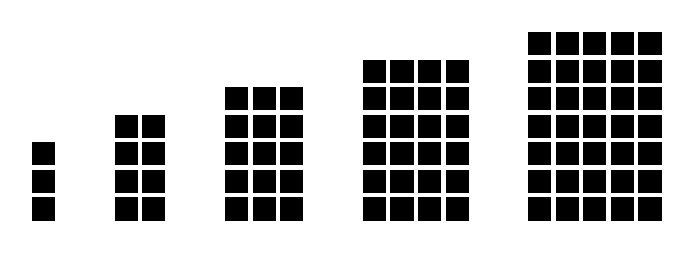
\begin{tikzpicture}[scale=0.35]
	\foreach \x in {0}
	\foreach \y in {0,...,2}
	\draw [ultra thick, white, fill=black] (\x,\y) rectangle (\x+1,\y+1);

	\begin{scope}[xshift=3cm]
	\foreach \x in {0,...,1}
	\foreach \y in {0,...,3}
	\draw [ultra thick, white, fill=black] (\x,\y) rectangle (\x+1,\y+1);
	\end{scope}

	\begin{scope}[xshift=7cm]
	\foreach \x in {0,...,2}
	\foreach \y in {0,...,4}
	\draw [ultra thick, white, fill=black] (\x,\y) rectangle (\x+1,\y+1);
	\end{scope}

	\begin{scope}[xshift=12cm]
	\foreach \x in {0,...,3}
	\foreach \y in {0,...,5}
	\draw [ultra thick, white, fill=black] (\x,\y) rectangle (\x+1,\y+1);
	\end{scope}

	\begin{scope}[xshift=18cm]
	\foreach \x in {0,...,4}
	\foreach \y in {0,...,6}
	\draw [ultra thick, white, fill=black] (\x,\y) rectangle (\x+1,\y+1);
	\end{scope}
\end{tikzpicture}
\caption{Some ``rectangular numbers'': $3, 8, 15, 24, 35, \dotsc$}
\label{fig:rects}
\end{figure}

\begin{figure}[!htbp]
\centering

\begin{tikzpicture}[scale=0.35]
	\draw [ultra thick, white, fill=black] (0,0) rectangle (1,1);

	\begin{scope}[xshift=3cm]
	\foreach \x in {0,...,1}
	\foreach \y in {0,...,1}
	\draw [ultra thick, white, fill=black] (\x,\y) rectangle (\x+1,\y+1);
	\end{scope}

	\begin{scope}[xshift=7cm]
	\foreach \x in {0,...,2}
	\foreach \y in {0,...,2}
	\draw [ultra thick, white, fill=black] (\x,\y) rectangle (\x+1,\y+1);
	\end{scope}

	\begin{scope}[xshift=12cm]
	\foreach \x in {0,...,3}
	\foreach \y in {0,...,3}
	\draw [ultra thick, white, fill=black] (\x,\y) rectangle (\x+1,\y+1);
	\end{scope}

	\begin{scope}[xshift=18cm]
	\foreach \x in {0,...,4}
	\foreach \y in {0,...,4}
	\draw [ultra thick, white, fill=black] (\x,\y) rectangle (\x+1,\y+1);
	\end{scope}
\end{tikzpicture}
\caption{The perfect squares: $1, 4, 9, 16, 25, \dotsc$}
\label{fig:squares}
\end{figure}

The perfect squares have a straightforward formula. If we let $f(x)$ represent the area of figure $x$, then the perfect squares are represented by the formula
\[f(x)=x^2.\]
This is the parent function of the quadratic family.

The rectangles in \cref{fig:rects} also have a formula. If we let $g(x)$ represent the area of figure $x$, then we might notice that figure $x$ is $x$ units wide and $(x+2)$ units tall. So these rectangles are represented by the formula
\[g(x) = x(x+2).\]
We can simplify this formula using the distributive property:
\[g(x) = x(x+2) = x^2 + 2x\]

We have learned that the highest degree term in a quadratic equation is an $x^2$ term. The connection between a quadratic rule and rectangles will help us when it comes to solving quadratic equations. In fact, we will solve these equations using the beautiful symmetry of the square.

% % % % % % % % % % % % % % % % % % % % % % % % % % % % % % % % % % % % % % % % 
\section{Level 1 and 2 quadratics}

As we did with linear equations, we'll treat quadratic equations like a game. Level 1 is the easiest kind of quadratic equation to solve, so this is where we'll start. Then, we'll keep things interesting as we increase our skill level by adding challenge and complexity along the way.

\subsection{Level 1 quadratics}

\begin{boxexplore}[Quadratic level 1]
Determine the value of $x$ given the equation: $x^2 = 64$.
\end{boxexplore} %% End of startup exploration

Talk about starting with the easy stuff. We're looking for a number $x$ which, when multiplied by itself, is equal to 64. In other words, we are looking for the ``square root of 64''. Clearly, $x=8$ is a solution to this equation. But we can't be too hasty! Notice that $x=\umin8$ is also a solution, since $(\umin8)^2 = (\umin8)(\umin8) = 64$. So, this equation has two solutions:
\[x = 8 \OR \umin8\]
If we prefer to write our answer in solution set notation, we have \[\solset{8,\umin8}.\]

So, Level 1 quadratics are pretty easy: we simply take the square root of both sides of the equation.\footnote{More soon on square roots, including why and under what circumstances ``square root of both sides'' is, in fact, a property of equality.} We might have a hard time if the constant value is not a perfect square, as in $x^2 = 12$. But, we'll learn more about handling the square roots of non-perfect-squares soon enough (in \cref{ch:radicals}, to be precise).

This seems like a good time to suggest that it may come in handy to memorize the first 25 or so perfect squares, for quick recognition when they come up in a problem.
\begin{align*}
1^2 &= 1		&
2^2 &= 4		&
3^2 &= 9		&
4^2 &= 16		&
5^2 &= 25		\\
6^2 &= 36		&
7^2 &= 49		&
8^2 &= 64		&
9^2 &= 81		&
10^2 &= 100	\\
11^2 &= 121	&
12^2 &= 144 	&
13^2 &= 169 	&
14^2 &= 196 	&
15^2 &= 225 	\\
16^2 &= 256 	&
17^2 &= 289 	&
18^2 &= 324 	&
19^2 &= 361 	&
20^2 &= 400 	\\
21^2 &= 441 	&
22^2 &= 484 	&
23^2 &= 529 	&
24^2 &= 576 	&
25^2 &= 625 	\\
\end{align*}

Finally, note that zero is also a perfect square, since $0^2 = 0$. Zero, in fact, is the only number that has only one square root. Whereas both 3 and $\umin3$ are square roots of 9, the only square root of 0 is 0.

Finally, consider the square root of a negative number, say, $\umin25$. This is a bit of a problem. We're meant to find the the number that when multiplied by itself gives $\umin25$ as the result, but that's not going to work. Since we have a negative product, the two factors must have opposite signs! The best we can do is $5\cdot\umin5 = \umin25$ or $\umin5\cdot5 = \umin25$, and in these cases we're not multiplying a number times itself: 5 and $\umin5$ are different numbers!

So, there is no real number equal to the square root of $\umin25$. Of course, $\umin25$ isn't special, the same argument applies to any negative number. The moral of the story is this: If, as we go about solving a quadratic equation, we come to the point where we need to take the square root of a negative number, we have to stop and say that the equation has ``no real number'' as its solution. $\mathcal{S}=\emptyset$.


\subsection{Level 2 quadratics}

\begin{boxexplore}[Quadratic level 2]
Determine the value of $w$ given the equation: $(w+3)^2 = 16$.
\end{boxexplore} %% End of startup exploration

Here, we're told that something-squared is 16. Well, that means that the something in question must either be 4 or negative 4. That is to say, $(w+3)$ is either 4 or $\umin4$. So, this equation is actually two equations at once. We have:
\[w+3 = 4 \qquad\text{\underline{or}}\qquad w+3 = -4\]
Solving these equations (using SPOE in both cases), we have that $w$ must be either $1$ or $\umin7$. So, those are our two solutions: $\solset{1,\umin7}$.

We can record this work in a down-the-page format, like so:
\begin{align*}
(w+3)^2 &= 16
\\
w+3 &= 4 \OR \umin4
&&\text{square root of both sides}
\\
w &= 1 \OR \umin7
&&\text{SPOE: subtract 3 throughout}
\end{align*}

A few things to note: First, we can't subtract 3 from both sides as the very first step. The parentheses require that we undo the exponent first. Second, beware the use of $\pm$. It may be tempting to use this shorthand notation and write
\begin{align*}
w+3 &= \pm4,\\
\intertext{but then it is also tempting to subtract 3 and write}
w &= \pm1. \quad\text{Nope!}
\end{align*}
We recommend splitting into two equations, or writing out the two solutions explicitly using the word ``or''.

\begin{boxex}
Determine the value of $a$ given the equation: $(a-1)^2 - 2 = 23$.

\exsoln\ This equation requires an extra step, but it's quickly transformed into an equation like the one from the startup exploration.
\begin{align*}
(a-1)^2 - 2 &= 23
\\
(a-1)^2 &= 25
&&\text{APOE}
\\
a-1 &= 5 \OR \umin5
&&\text{square root of both sides}
\\
w &= 6 \OR \umin4
&&\text{APOE: add 1 throughout}
\end{align*}
In the end, we have $\solset{6, \umin4}$.
\end{boxex}

% % % % % % % % % % % % % % % % % % % % % % % % % % % % % % % % % % % % % % % % 
\section{Level 3 quadratics: Quadrangle method}

\begin{boxexplore}[Quadratic level 3]
Use the sum to a power property (from \cref{sec:exposumstopowers}) to write the expression $(x+3)^2$ without parentheses. Then, determine the value of $x$ given the equation: $x^2+6x+9 = 49$.
\end{boxexplore} %% End of startup exploration

To expand $(x+3)^2$, we might think of using algebra tiles to fill in a square with side length $(x+3)$. We used algebra tiles to solve this kind of problem back in \cref{sec:exposumstopowers}. Or, we could just ``sketch'' the algebra tiles diagram (shown below, on the right) and calculate the areas of the four regions.

\begin{minipage}{0.49\linewidth}
\centering
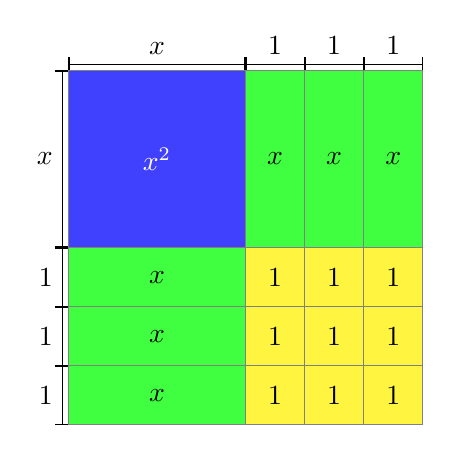
\begin{tikzpicture}[scale=0.75]
	\draw[|-|] (0,0.1) -- node[above]{$x$} (3,0.1);
	\draw[|-|] (-0.1,0) -- node[left]{$x$} (-0.1,-3);
	\draw[gray, fill=blue!75] (0,0) rectangle node[white]{$x^2$} (3,-3);
	\foreach \x in {3,...,5} {
		\draw[|-|] (\x,0.1) -- node[above]{1} (\x+1,0.1);
		\draw[gray, fill=green!75] (\x,0) rectangle node[black]{$x$} (\x+1,-3);
	}
	\foreach \y in {-3,...,-5} {
		\draw[|-|] (-0.1,\y) -- node[left]{1} (-0.1,\y-1);
		\draw[gray, fill=green!75] (0,\y) rectangle node[black]{$x$} (3,\y-1);
	}
	\foreach \x in {3,...,5} {
		\foreach \y in {-3,...,-5}
			\draw[gray, fill=yellow!75] (\x, \y) rectangle node[black]{1} (\x+1,\y-1);
	}
\end{tikzpicture}
\end{minipage}
%%
\begin{minipage}{0.49\textwidth}
	\quadrangle{x}{3}{x^2}{3x}{9}
\end{minipage}

Note how we have simplified the picture in the ``sketch'' version. For example, rather than draw three 3-unit-by-$x$-unit rectangles, we simply write the area of the rectangle $3x$. In the lower right-hand region, we write the area 9 rather than draw nine yellow squares.

We'll call this simplified sketch a \textit{quadrangle diagram}, and we'll call the method we are developing here the \textit{quadrangle method}.\footnote{The term \textit{quadrangle} is a synonym for \textit{rectangle}. History suggests that the term \textit{quadratic} is related to the term \textit{quadrangle} since this method of using square diagrams is so helpful in solving quadratic equations.} The quadrangle diagram can help us to see the relationship between the two expressions in the startup exploration:
\[(x+3)^2 = x^2 + 6x + 9.\]
Using this fact, we can solve the given equation:
\begin{align*}
x^2 + 6x + 9 &= 49
\\
(x+3)^2 &= 49
&&\text{based on the quadrangle diagram}
\\
x+3 &= 7 \OR \umin7
&&\text{square root of both sides}
\\
x &= 4 \OR \umin10
&&\text{SPOE: subtract 3 throughout}
\end{align*}
Can you see the clever trick that we used here? We rewrote an expanded expression as a something-squared expression, and then we solved it like a Level 2 quadratic!

Let's work through another example in detail, for example, solving the Level 3 equation
\[x^2 + 12x + 36 = 144.\]

Our goal is to write the left-hand side in a something-squared form. To do that, we'll begin by drawing an empty quadrangle diagram and filling in the bits that we know. For example, we know that the upper left-hand box must contain $x^2$, and so the sides of that square must each be $x$ units long.

\quadrangle{x}{}{x^2}{}{}

We know that the 36 will appear in the lower right-hand box. But how sould we label the side lenghts here? There are lots of combinations of numbers that multiply together to get 36\ldots

\quadrangle{x}{?}{x^2}{}{36}

Remember that the goal is to get an expression of the form something-\textit{squared}, and so we should always strive to create a quadrangle that is, in fact, a square. This means that we must choose 6 and 6 as the side lengths. If we chose another pair of factors, like 2 and 18, we would get the proper product in the lower right-hand region, but our overall diagram would no longer be a square.

\quadrangle{x}{6}{x^2}{}{36}

To fill in the remaining regions, we multiply the dimensions of each. In both cases we get $6x$. This is good news! Together these make $12x$ (which is what we have in the original, expanded expression). Plus, the two regions contain the same value, and so the beautiful symmetry of the square is preserved.

\quadrangle{x}{6}{x^2}{6x}{36}

So, we have rewritten our expression as a something-squared expression:
\[x^2 + 12x + 36 = (x+6)^2.\]
We can use this to solve the equation that we were given:
\begin{align*}
x^2 + 12x + 36 &= 144
\\
(x+6)^2 &= 144
&&\text{based on the quadrangle diagram}
\\
x+6 &= 12 \OR \umin12
&&\text{square root of both sides}
\\
x &= 6 \OR \umin18
&&\text{SPOE}
\end{align*}

\begin{boxex}
Determine the value of $n$ given the equation: $n^2 - 16n + 64 = 1$.

\exsoln\ Let's build the quadrangle diagram. The upper left-hand corner contains $n^2$, as above. To maintain symmetry, we should split the $-16n$ exactly in half. Don't worry about the negative coefficient, we can work with that. We should be on guard though for sign-related issues.

\quadrangle{n}{}{n^2}{-8n}{}

This tells us that the remaining portion of the square's side length must be $-8$. Let's not worry too much about the fact that negative distances are impossible\ldots\ the idea still works. This implies that the remaining region contains 64 (note, that positive 64). This agrees with the equation we were given.

\quadrangle{n}{-8}{n^2}{-8n}{64}

Now, we can solve the equation:
\begin{align*}
n^2 -16n +64 &= 1
\\
(n-8)^2 &= 1
&&\text{based on the quadrangle diagram}
\\
n-8 &= 1 \OR \umin1
&&\text{square root of both sides}
\\
n &= 9 \OR 7
&&\text{SPOE}
\end{align*}
So, we have $\solset{7,9}$. We can check our work by substituting our proposed solutions back into the original equation. First, we'll test $n=7$:
\begin{align*}
n^2 -16n +64 &= 1
\\
(7)^2 - 16(7) + 64 &\overset{?}{=} 1
\\
49 - 112 + 64 &\overset{?}{=} 1
\\
1 &\overset{\checkmark}{=} 1
\end{align*}
First, we'll check $n=9$:
\begin{align*}
n^2 -16n +64 &= 1
\\
(9)^2 - 16(9) + 64 &\overset{?}{=} 1
\\
81 - 144 + 64 &\overset{?}{=} 1
\\
1 &\overset{\checkmark}{=} 1
\end{align*}
\end{boxex}

% % % % % % % % % % % % % % % % % % % % % % % % % % % % % % % % % % % % % % % % 
\section{Level 4 quadratics: Adjust the constant term}

\begin{boxexplore}[Quadratic level 4]
Determine the value of $x$ given the equation: $x^2 + 8x + 15 = 99$.
\end{boxexplore} %% End of startup exploration

Let's try to build the quadrangle diagram. The upper left-hand corner contains $x^2$, as before. To maintain symmetry, we should split the $8x$ exactly in half. This tells us that the large square must be $(x+4)$ units on a side.

\quadrangle{x}{4}{x^2}{4x}{}

The problem is that, according to our quadrangle diagram, the lower right-hand corner should be 16\ldots\ but the equation we are given tells us to put 15 in that space. Now what? Our equation does not represent a complete square!

\quadrangle{x}{4}{x^2}{4x}{\color{red}15}

POEs to the rescue! Why not add 1 to both sides of the given equation to complete the square? This will give us the number we want on the left-hand side and, since we add 1 to both sides, we have an equivalent equation. So, instead of solving the equation
\[x^2 + 8x + 15 = 99,\]
we will add one to both sides and solve the equation
\[x^2 + 8x + 16 = 100.\]
Now, we can draw the quadrangle diagram exactly as we wanted.

\quadrangle{x}{4}{x^2}{4x}{16}

And now that we have a proper quadrangle diagram, we can solve the equation! Here's the full process:
\begin{align*}
x^2 + 8x + 15 &= 99
\\
x^2 + 8x + 16 &= 100
&&\text{APOE: add 1 to both sides}
\\
(x+4)^2 &= 100
&&\text{based on the quadrangle diagram}
\\
x+4 &= 10 \OR \umin10
&&\text{square root of both sides}
\\
x &= 6 \OR \umin14
&&\text{SPOE}
\end{align*}

This is a clever application of the POEs. Rather than use the properties to eliminate terms from one side of the equation, we can use the properties to change one side into a particular, more-helpful form.\footnote{In fact, this is exactly what we've been doing all along: changing one side of an equation into a form that is more helpful. In this chapter we are expanding our notion of what it means for a change to be ``helpful''.}

\begin{boxex}
Determine the value of $x$ given the equation: $x^2-6x+11=27$.

\exsoln\ When we start the quadrangle diagram, we split the $-6x$ as usual. This means that the square has sides of length $(x-3)$. This, in turn, implies that the lower right-hand region should be 9. Our equation has 11 as its constant term: not what we want.

\quadrangle{x}{-3}{x^2}{-3x}{\color{red}9}

To fix, this we can subtract 2 to each side of our equation. This will give us a constant term of 9, which is what we need to make our quadrangle diagram work. So, we have:
\begin{align*}
x^2 - 6x + 11 &= 27
\\
x^2 - 6x + 9 &= 25
&&\text{SPOE: subtract 2 from both sides}
\\
(x-3)^2 &= 25
&&\text{based on the quadrangle diagram}
\\
x-3 &= 5 \OR \umin5
&&\text{square root of both sides}
\\
x &= 8 \OR \umin2
&&\text{SPOE}
\end{align*}
So, our solutions are $\solset{8, \umin2}$.
\end{boxex}

% % % % % % % % % % % % % % % % % % % % % % % % % % % % % % % % % % % % % % % % 
\section{Level 5 quadratics: Adjust the linear term}

The last few levels have had ``polite'' middle terms, which have split evenly into two pieces. What happens if we get a linear term with an odd coefficient?

\begin{boxexplore}[Quadratic level 5]
Determine the value of $x$ given the equation: $x^2 + 3x + 1 = 5$.
\end{boxexplore} %% End of startup exploration

If we jump right in and try the quadrangle method, we start to get into fraction territory. If we want to split the $3x$ term exactly in half, then each piece would be $\frac{3}{2}$. Then, the quadrangle method would predict $\frac{9}{4}$ in the lower-right corner.

\quadrangle{x}{\frac{3}{2}}{x^2}{\frac{3}{2}x}{\color{red}\frac{9}{4}}

The lower-right corner isn't what we have in our equation, so we could use APOE and add $\frac{5}{4}$ to adjust both sides\ldots\ Hmm. Not pretty. To be clear, the quadrangle method will not let us down: if we keep going with the fractions, we will arrive at the correct answer! But, perhaps there is an alternative approach that avoids the fractions.

Here's a clever idea: We could use MPOE and multiply through by 2. This would give us a linear term with an even coefficient! In other words:
\[x^2 + 3x + 1 = 5 \quad\xrightarrow{\quad\text{multiply through by 2}\quad}\quad 2x^2 + 6x + 2 = 10\]
This fixes our odd coefficient problem, since now we can break the $6x$ up into two sets of $3x$. But, what do we do with that $2x^2$? We can't use $x$ and $2x$ as the side lengths, for although that gives is the correct product, we would no longer have a square.

\quadrangle{\color{red}?}{3}{2x^2}{3x}{}

Now, here's a \textit{really} clever idea. Let's multiply through by 2 \textit{again}. In other words, we will multiply the original equation by 4:
\[x^2 + 3x + 1 = 5 \quad\xrightarrow{\quad\text{multiply through by 4}\quad}\quad 4x^2 + 12x + 4 = 20\]
We still have an even linear coefficient, and now we can write $4x^2$ as $2x$ times $2x$. Note that we have to take that factor of 2 into account when we're figuring out the other dimensions of the square. Study our new diagram closely and be sure you understand where each of the labels comes from.
\begin{center}
	\quadrangle{2x}{3}{4x^2}{6x}{9}
\end{center}

We now find ourselves in a Level 4 situation: our equation has 4 as the constant term, whereas the quadrangle diagram predicts 9 as the constant term. No problem! We can add 5 to both sides, and continute the process as we did with Level 4 quadratics. Here's a summary of the whole process:
\begin{align*}
x^2 + 3x + 1 &= 5
&&\text{original equation}
\\
4x^2 + 12x + 4 &= 20
&&\text{MPOE: multiply both sides by 4}
\\
4x^2 + 12x + 9 &= 25
&&\text{APOE: add 5 to both sides}
\\
(2x+3)^2 &= 25
&&\text{based on the quadrangle diagram}
\\
2x+3 &= 5 \OR \umin5
&&\text{square root of both sides}
\\
2x &= 2 \OR \umin8
&&\text{SPOE}
\\
x &= 1 \OR \umin4
&&\text{DPOE}
\end{align*}

Let's pause and review. When faced with an odd coefficient for the $x$ term, our strategy is to multiply through by 4. This will give us an even coefficient for the $x$ term, and at the same time keep the coefficient of the $x^2$ term in a state where it can be written as something times itself: $4x^2 = 2x\cdot2x$. After we do this, we'll have a Level 4 quadratic on our hands, and we can apply techniques for handling those.

\begin{boxex}
Determine the value of $x$ given the equation: $x^2-5x+12=62$.

\exsoln\ Faced with an odd linear coefficient, we multiply through by 4. This gives us the revised equation \[4x^2-20x+48=248.\] We set up the quadrangle diagram and see whether our equation represents a complete square.

\quadrangle{2x}{-5}{4x^2}{-10x}{\color{red}25}

Our (revised) equation does not make a proper square: the constant term in the equation is 48, but the quadrangle diagram predicts 25. We can fix this problem using SPOE: subtract 23 from both sides:
\begin{align*}
x^2 - 5x + 12 &= 62
&&\text{original equation}
\\
4x^2 - 20x + 48 &= 248
&&\text{MPOE: multiply both sides by 4}
\\
4x^2 - 20x + 25 &= 225
&&\text{SPOE: subtract 23 from to both sides}
\\
(2x-5)^2 &= 225
&&\text{based on the quadrangle diagram}
\\
2x-5 &= 15 \OR \umin15
&&\text{square root of both sides}
\\
2x &= 20 \OR \umin10
&&\text{SPOE}
\\
x &= 10 \OR \umin5
&&\text{DPOE}
\end{align*}
So in the end, we have solutions $\solset{10, \umin5}$.
\end{boxex}

% % % % % % % % % % % % % % % % % % % % % % % % % % % % % % % % % % % % % % % % 
\section{Level 6 quadratics: Adjust the quadratic term}

We've arrived at the highest level of the quadratic equation challenge! Until now, all of our equations have started with just $x^2$. What if the coefficient of the leading term is something other than 1?

\begin{boxexplore}[Quadratic level 6]
Determine the value of $x$ given the equation: $3x^2 + 8x + 1 = 12$.
\end{boxexplore} %% End of startup exploration

What shall we do in this scenario? A clever idea is to use DPOE and divide through by 3. That would make the leading coefficient 1, as in the earlier problems. The downside is that most of the other numbers turn into fractions.
\[3x^2 + 8x + 1 = 12
\quad\xrightarrow{\quad\text{divide through by 3}\quad}\quad
x^2 + \frac{8}{3}x + \frac{1}{3} = 4\]
The quadrangle method will absolutely work on an equation like this, but perhaps we'd prefer an approach that avoided all the fractions.

If scaling the equation down doesn't help, why not try to scale it up? Could we multiply through by some helpful value? Recall that the goal will be to write the $x^2$ term as something times itself. Since there's already a 3 there, we can solve our problem if we multiply through by 3.
\[3x^2 + 8x + 1 = 12
\quad\xrightarrow{\quad\text{multiply through by 3}\quad}\quad
9x^2 + 24x + 3 = 36\]
Note that now we are in a good position, since $9x^2 = 3x\cdot3x$. So, let's fill out our quadrangle diagram. We have an even coefficient on the linear term, so we can split that evenly. Note that we have to take all the coefficients into account when completing the diagram. For example, when figuring out the dimensions of a box containing $12x$.

\quadrangle{3x}{4}{9x^2}{12x}{\color{red}16}

The quadrangle diagram predicts 16 as the constant term, and so our equation is not a complete square. We can use APOE to fix that, adding 13 to both sides. Here's how it goes:
\begin{align*}
3x^2 +8x + 1 &= 12
&&\text{original equation}
\\
9x^2 + 24x + 3 &= 36
&&\text{MPOE: multiply through by 3}
\\
9x^2 +24x + 16 &= 49
&&\text{APOE: add 13 to both sides}
\\
(3x+4)^2 &= 49
&&\text{based on the quadrangle diagram}
\\
3x+4 &= 7 \OR \umin7
&&\text{square root of both sides}
\\
3x &= 3 \OR \umin11
&&\text{SPOE}
\\
x &= 1 \OR \umin\tfrac{11}{3}
&&\text{DPOE}
\end{align*}

In summary, we multiplied through by the coefficient of the $x^2$ term, which gave us a coefficient that was a perfect square. In the final example for this chapter, we put it all together.

\begin{boxex}
Determine the value of $x$ given the equation $-5x^2-x+18=0$.

\exsoln\ Since we have a leading coefficient that is not a perfect square, we multiply through by that coefficient, $-5$ in this case. This gives us
\[25x^2+5x-90=0\]
(careful with the negative signs). This is an improvement, but we have a linear coefficient that is odd. So, we multiply by 4 to fix that:
\[100x^2 + 20x - 360=0\]
Notice that multiplying through by 4 (a perfect square) gives us a leading coefficient that is still a perfect square. This is because the product of two perfect squares is itself a perfect square! (Can you prove that this statement is always true using the properties of exponents?)

We now have a revised equation that we can bring to the quadrangle method.

\quadrangle{10x}{1}{100x^2}{10x}{\color{red}1}

To get our constant terms to agree, we must add 361 to both sides of our revised equation. This gives us
\[10x^2 + 10x + 1 = 361.\]
And from here, we can complete a familiar process.
\begin{align*}
10x^2 +10x + 1 &= 316
&&\text{}
\\
(10x+1)^2 &= 316
&&\text{based on the quadrangle diagram}
\\
10x+1 &= 19 \OR \umin19
&&\text{square root of both sides}
\\
10x &= 18 \OR \umin20
&&\text{SPOE}
\\
x &= \tfrac{18}{10} \OR \umin2
&&\text{DPOE}
\end{align*}
After we simplify our one fraction answer, we have a final solution: $\solset{\frac{9}{5}, \umin2}$.
\end{boxex}

\subsection{(;,;) Quadratic formula}
\label{sec:quadformulapreview}

Now that we have the quadrangle method at our disposal, we can tackle any quadratic equation that is thrown at us. We might be tempted to really get generic, and solve the all at once.

Consider a completely generic quadratic equation of the form \[ax^2 + bx + c=0.\] This quadratic has three coefficients: $a$ is the coefficient of the quadratic term, $b$ is the coefficient of the linear term, and $c$ is the constant term. We've set it equal to zero for reasons that will be made clear in a few chapters.\footnote{Sorry for the mystery, but all will be revealed soon. In the meantime, note that we can always turn a quadratic equation into this form. If we have an equation that does not equal zero, for example $ax^2 + bx + c = d$ where $d$ is not zero, then we can use SPOE to get 0 on the right-hand side: $ax^2+bx+c-d=0$. Then, we pull a little algebraic sleight of hand, and replace $c-d$ with just $c$. This might look like an illegal move, but in the general form of a quadratic, ``$c$'' just stands for a constant value. Since ``c-d'' is a contstant value, we pretend that this was the constant value we meant all along.}

What happens if we apply the quadrangle method to this totally generic equation? We don't really know anything about $a$, so to be safe, let's multiply the whole equation by $a$. 
\[a^2x^2 + abx + ac=0.\]
This will ensure that the leading term is a perfect square, and that's what we need for the box method. Now, the linear coefficient is $ab$ and this might be an odd number for all we know. So, we multiply through by 4, as we have often done above.
\[4a^2x^2 + 4abx + 4c=0.\]
This is not a pretty sight, but we'll try to make it work with the quadrangle method.

\quadrangle{2ax}{b}{4a^2x^2}{2abx}{\color{red}b^2}

Much of this looks workable, but what about the lower right-hand corner? The quadrangle method predicts $b^2$, but our equation has $4c$. Well, we'll do what we usually do: we'll use the POEs to turn our left-hand side into the form we want. So:

\begin{align*}
4a^2x^2 + 4abx + 4c &= 0
&&\text{}
\\
4a^2x^2 + 4abx &= -4c
&&\text{SPOE: subtract $4c$ from both sides}
\\
4a^2x^2 + 4abx +b^2 &= b^2-4c
&&\text{APOE: add $b^2$ to both sides}
%
\intertext{It might seem like things are getting worse, but now the left-hand side is what we need to use our quadrangle diagram. Let's go!}
%
(2ax+b)^2 &= b^2-4c
&&\text{based on the quadrangle diagram}
\\
2ax+b &= \pm\sqrt{b^2-4c}
&&\text{square root of both sides}
\\
2ax &= \pm\sqrt{b^2-4c}-b
&&\text{SPOE: subtract $b$ from both sides}
\\[1ex]
x &= \frac{\pm\sqrt{b^2-4c}-b}{2a}
&&\text{DPOE: divide both sides by $2a$}
\\[1ex]
x &= \frac{-b\pm\sqrt{b^2-4c}}{2a}
&&\text{rearranging the numerator}
\end{align*}

That last rearrangement in the numerator is because it looks a little better, and to make it clear that the $-b$ isn't underneath the radical along with that other stuff. Also, it's tradition. This formula is a famous thing, and traditionally appears in this form.

% % % % % % % % % % % % % % % % % % % % % % % % % % % % % % % % % % % % % % % % 
\chaptersummary

The properties of equality which we learned before this chapter weren't enough to solve any random quadratic equation. To overcome the quadratic obstacle, we learned new techniques for solving quadratic equations. These new techniques are based on the symmetry of a square, and we learned various techniques for adjusting a quadratic equation so that we can use our new quadrangle method.

We have, however, avoided the necessity of finding the square root of a number that was not a perfect square. This was a helpful simplification -- it allowed us to focus on the process of equation solving -- but not all quadratics will have answers that come out so ``nice''. We turn our attention to square roots in the next chapter.
